\begin{frame}{Experimental Study: Optimizations}
    We proposed different optimizations that could be applied to the \DPmst.
    \begin{itemize}
        \item Multiple roots per filter
        \item Decoupled Event Handling
        \item Adaptive \mst\ Caching
        \item Memory management
        \item Preprocessing
    \end{itemize}
\end{frame}

\begin{frame}{Experimental Study: Decoupled Event Handling (I)}
    \justifying
    MST is more costly than other operations. This can hold all the incoming operations although they are not related. A possible solution: separate operation reception and data structures modification.

    \textcolor{white}{Here goes some text}
    %\linebreak

    \begin{columns}
    \column{0.4\textwidth}
    \begin{tikzpicture}
        \begin{pgfonlayer}{stages}
            \node [style=filter_gen, minimum width=1cm, minimum height=3cm] (1) at (0, 0) {Filter};

            %Before
            \draw [style={opChan}] ([yshift=0.5 cm,xshift=-1.25cm]1.west) to["Op"] ([yshift=0.5 cm]1.west);
            \draw [style={daChan}] ([yshift=-0.5 cm,xshift=-1.25cm]1.west) to["Data"] ([yshift=-0.5 cm]1.west);

            %After
            \draw [style={opChan}] ([yshift=0.5 cm]1.east) to["Op"] ([yshift=0.5 cm,xshift=1.25cm]1.east);
            \draw [style={daChan}] ([yshift=-0.5 cm]1.east) to["Data"] ([yshift=-0.5 cm,xshift=1.25cm]1.east);
        \end{pgfonlayer}
        \begin{pgfonlayer}{edgelayer}
        \end{pgfonlayer}
    \end{tikzpicture}
    \column{0.4\textwidth}
    \begin{tikzpicture}
        \begin{pgfonlayer}{stages}
            \node [style=filter_gen, minimum width=1.75cm, minimum height=3cm] (1) at (0, 0) {};
            \node [style=filter_gen, minimum width=1cm, minimum height=1cm] (MailBox) at (0, 0.8) {MailBox};
            \node [style=filter_gen, minimum width=1cm, minimum height=1cm] (Worker) at (0, -0.8) {Worker};

            %Before
            \draw [style={opChan}] ([xshift=-1.25cm]MailBox.west) to["Op"] (MailBox.west);
            \draw [style={daChan}] ([xshift=-1.25cm]Worker.west) to["Data"] (Worker.west);

            % Between
            \draw [style={opChan}] (MailBox.south) to["Op"] (Worker.north);

            %After
            \draw [style={opChan}] (MailBox.east) to["Op"] ([xshift=1.25cm]MailBox.east);
            \draw [style={daChan}] (Worker.east) to["Data"] ([xshift=1.25cm]Worker.east);
        \end{pgfonlayer}
        \begin{pgfonlayer}{edgelayer}
        \end{pgfonlayer}
    \end{tikzpicture}
    \end{columns}
\end{frame}

\begin{frame}{Experimental Study: Decoupled Event Handling (II)}
    We generated instances with different number of operations and measure the execution time of \DPmst\ of different file sizes with and without the MailBox/Worker optimization.

    \begin{table}[H]
        \centering
        \begin{tabular}{@{}lrr@{}}
        \toprule
        Operations & No optimization & With optimization \\ \midrule
        7500       & 1h 9m 31.48s    & 57m 28.23s        \\
        10000      & 3h 46m 46.73s   & 2h 44m 14.19s     \\ \bottomrule
        \end{tabular}
    \end{table}
\end{frame}


\begin{frame}{Experimental Study: Comparison}
    \centering
    \begin{tikzpicture}
        \node  (0) at (0, 0) {Experimental Study};
        \node [below left=1cm and 0.5cm of 0] (1) {Static Case};
        \node [below right=1cm and 0.5cm of 0] (2) {Dynamic Case};
        \node [below=1cm of 1] (3) {Random Graphs};
        \node [below=1cm of 2] (4) {Real Graphs};
        \draw[style={tree_edge}]{} (0) to (1);
        \draw[style={tree_edge}]{} (0) to (2);
        \draw[style={tree_edge}]{} (1) to (3);
        \draw[style={tree_edge}]{} (2) to (4);
    \end{tikzpicture}
    
    \textcolor{white}{Here goes some text}
    
    \justifying
    We measured elapsed wall-clock time $T(k,n,p)$ and we refer to  absolute speed up and efficiency as: 
    \begin{itemize}
        \item \textit{Absolute speedup}: $speedup_a(k) = T(1, n, p)/T(k, n, p)$.
        \item \textit{Efficiency}: $speedup_a(k)/k$.
    \end{itemize} 

\end{frame}

\begin{frame}{Experimental Study: Static Case (I)}
    20 static binomial random graphs for each combination of:
    \begin{itemize}
        \item Number of vertices: $n \in \{ 10^3, 2\cdot10^3, 10^4, 5\cdot10^4 \}$
        \item Edge probability: $p \in \{ 0.25, 0.50, 0.75, 0.90\}$
    \end{itemize}

\end{frame}

\begin{frame}{Experimental Study: Static Case (II)}
    \begin{figure}
            \centering
            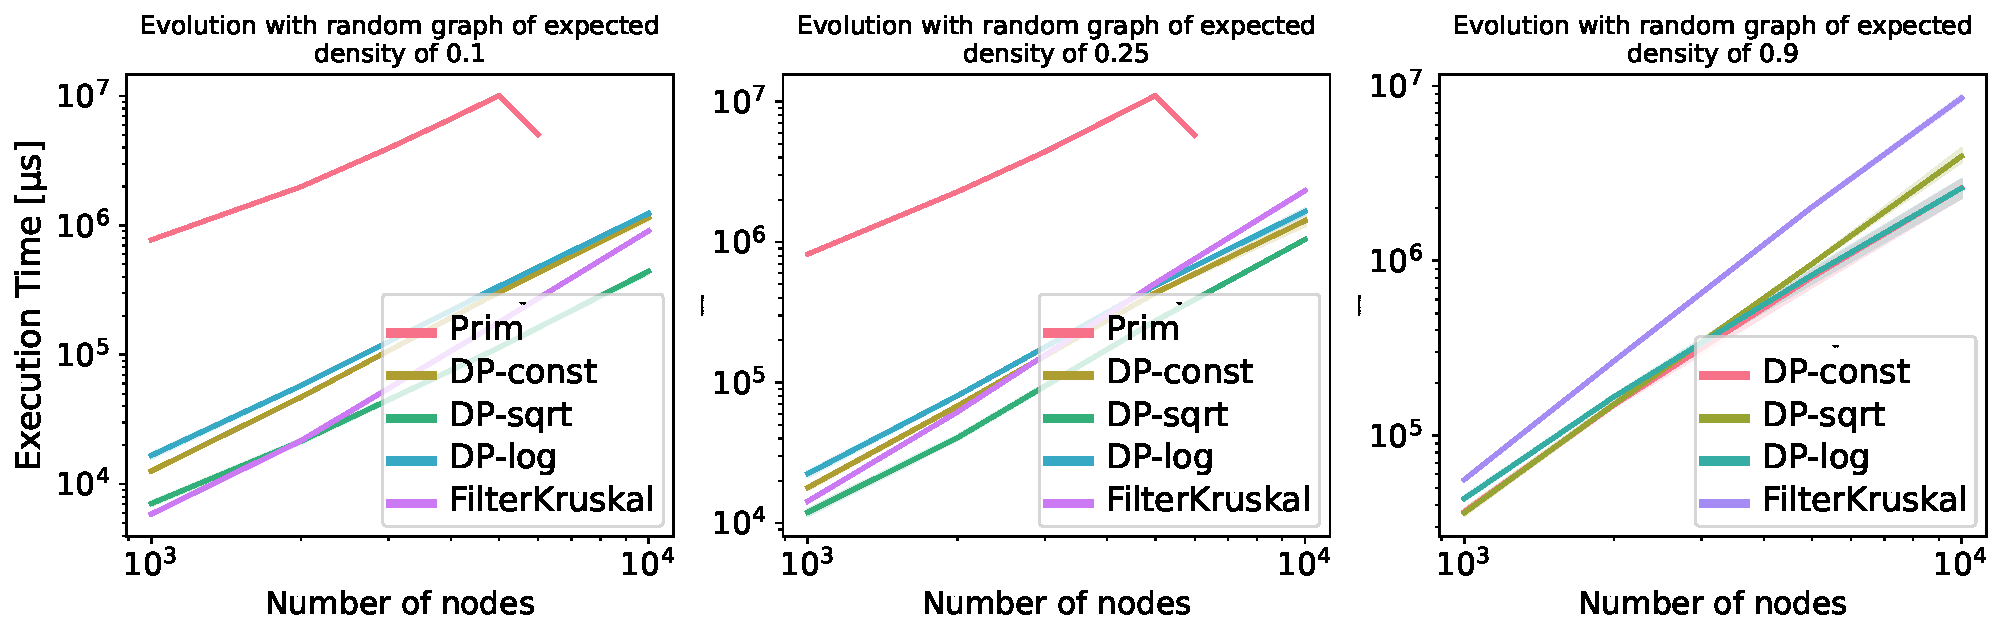
\includegraphics[width=1\linewidth]{figures/SomeDensities_mixed.pdf}
    \end{figure}

    \begin{figure}
            \centering
            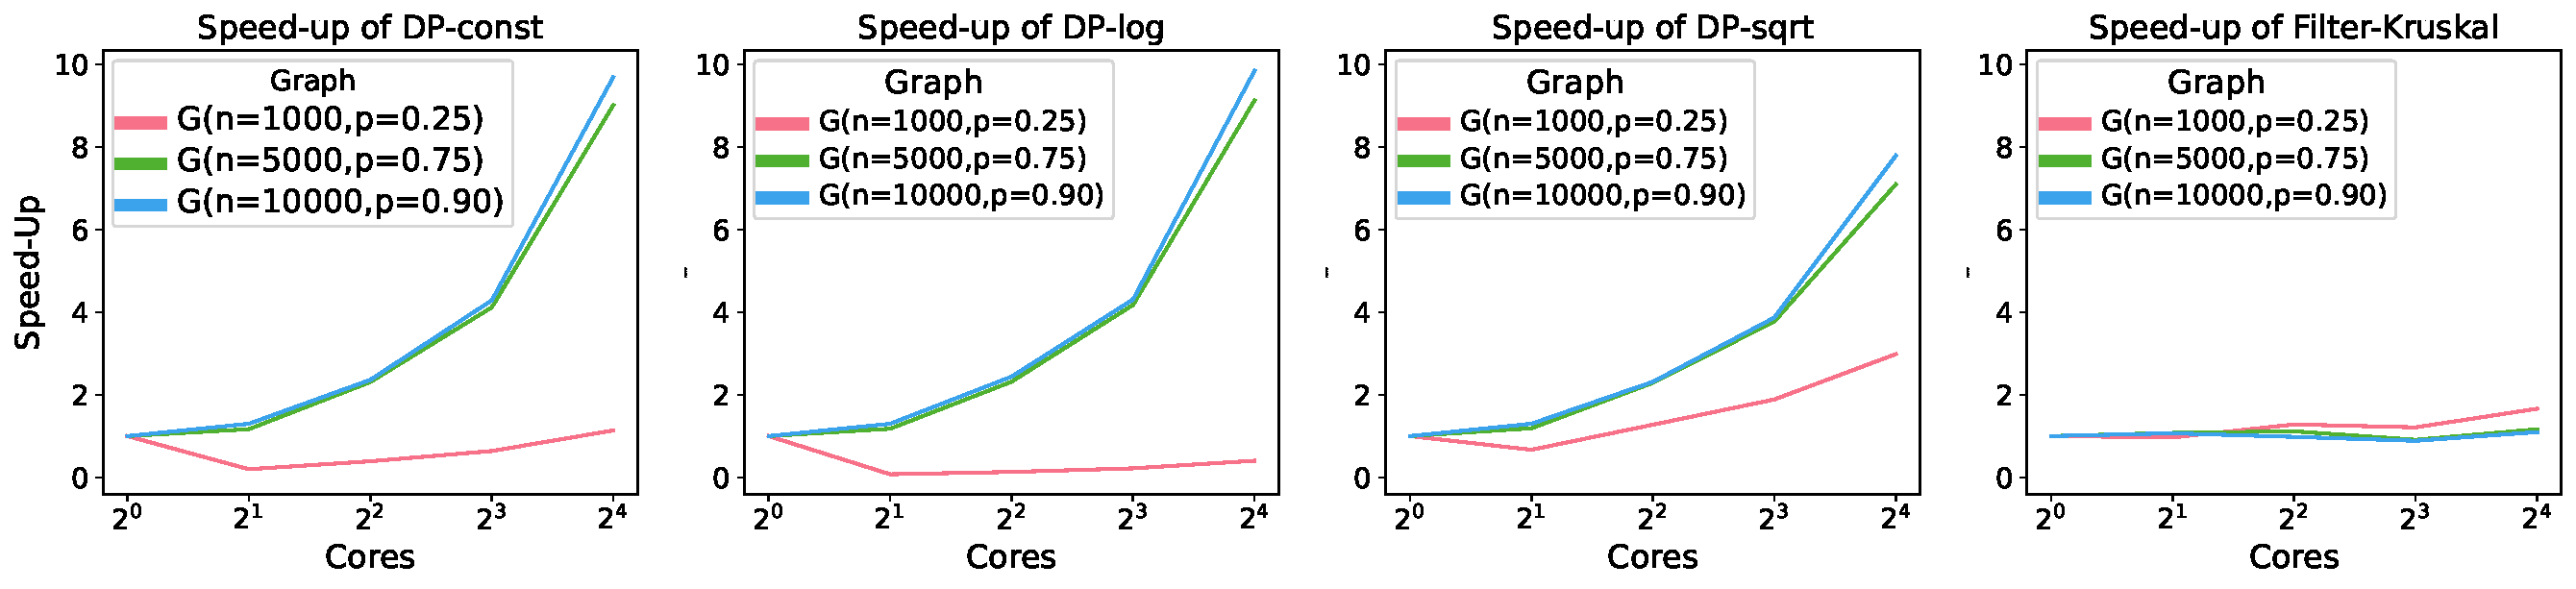
\includegraphics[width=1\linewidth]{figures/SpeedUpDPandFK_sample.pdf}
    \end{figure}
\end{frame}

\begin{frame}{Experimental Study: Dynamic case (I)}
We obtained some realistic dynamic graphs collected from a public repository.~\footnote{\href{https://DynGraphLab.github.io/}{\texttt{https://DynGraphLab.github.io/}}}. 

\begin{table}[H]
\centering
\begin{tabular}{@{}llll@{}}
\toprule
Dataset        & Vertices  & Operations & Density \\ \midrule
amazon-ratings & 495,452   & 476,728    & $1.94\cdot10^{-6}$ \\
as-caida       & 31,379    & 19,468     & $1.21\cdot10^{-4}$ \\
frwiki         & 2,212,682 & 31,624,375 & $6.46\cdot10^{-6}$ \\
movielens10m   & 49,847    & 384,585    & $1.55\cdot10^{-4}$ \\
simplewiki     & 100,312   & 889,016    & $8.84\cdot10^{-5}$ \\ \bottomrule
\end{tabular}
\end{table}
\end{frame}

\begin{frame}{Experimental Study: Dynamic case (II)}
    \begin{table}[]
    \centering
    \begin{tabular}{lrrr}
        \toprule
        Dataset            & \FKruskal & \DPmst\   & SpeedUp \\ \midrule
        {\tt as-caida}     &  1h 30min &  1h 19min & 1.14    \\
        {\tt movielens10m} &  1h 39min &  1h 20min & 1.24    \\
        {\tt simplewiki}   & 17h  8min & 11h 29min & 1.48    \\
        \bottomrule
    \end{tabular}
    \end{table}

    \begin{figure}
        \centering
        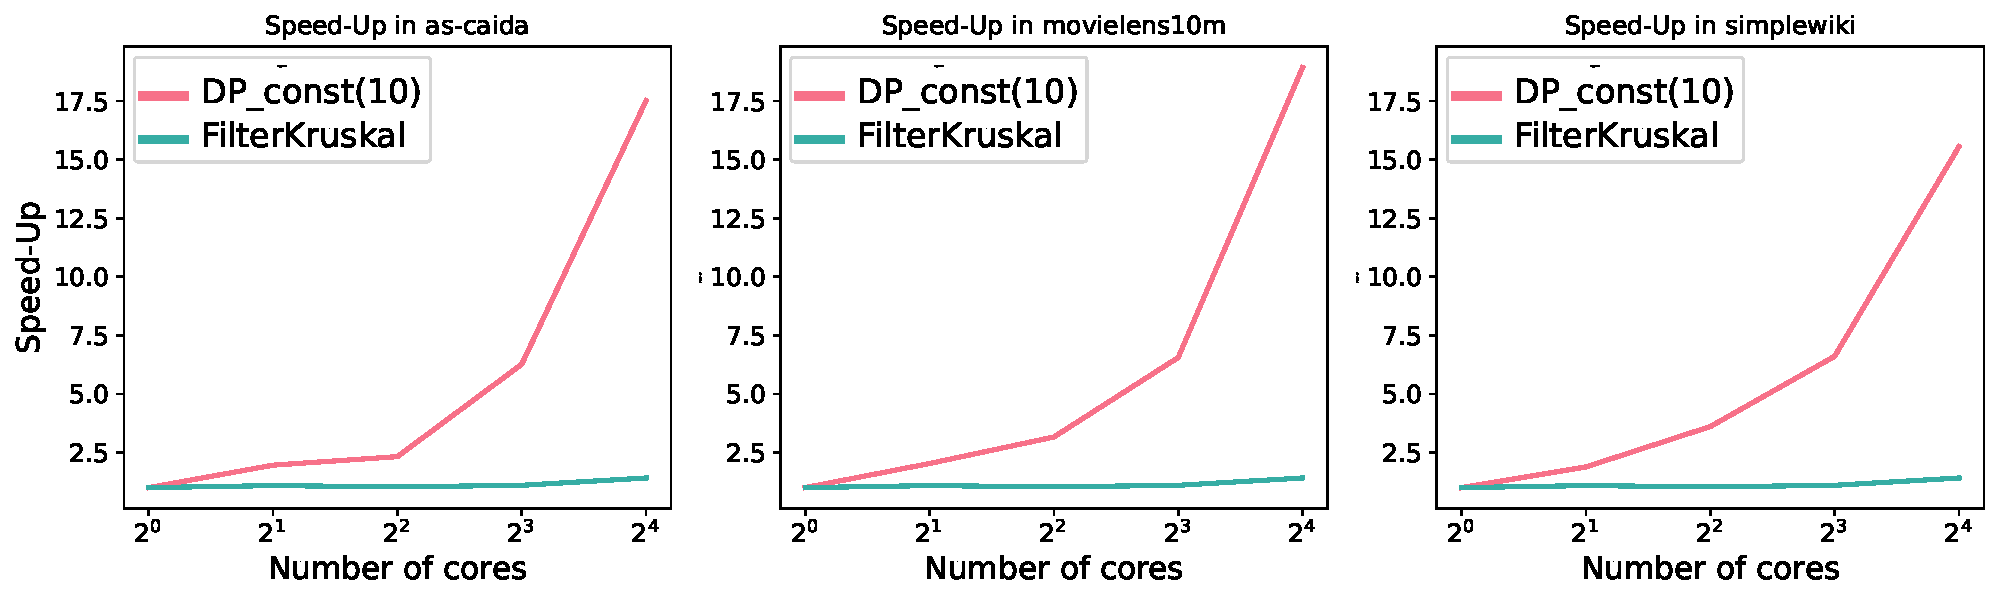
\includegraphics[width=\textwidth]{figures/RealGraphs.pdf}
    \end{figure}
\end{frame}